% blog-title: Change of Measure for Bandit Lower Bounds
% blog-date: 2026-06-20
% blog-description: A polished note on how nearby alternative worlds force evidence gathering, sample-complexity lower bounds, and Lai-Robbins style regret limits.
% blog-lang: en

\documentclass[en,nofont,11pt]{elegantbook}

\title{Change of Measure for Bandit Lower Bounds}
\subtitle{How Nearby Worlds Force Every Algorithm to Gather Evidence}
\author{Tang}
\institute{Tang's Machine Learning Blog}
\date{2026-06-20}
\version{1.0.0}
\bioinfo{Topic}{Change of Measure, Best-Arm Identification, Regret Lower Bounds}
\extrainfo{A LaTeX-native research note with reproducible simulations and code.}
\cover{assets/blog-cover.jpg}

\usepackage{fontspec}
\ifdefined\setCJKmainfont
\else
  \usepackage[UTF8,scheme=plain,fontset=none]{ctex}
\fi
\usepackage{xcolor}
\usepackage{listings}
\usepackage{float}
\usepackage{tcolorbox}
\tcbuselibrary{breakable, listings, skins}
\usetikzlibrary{arrows.meta,positioning,calc,decorations.pathmorphing,decorations.pathreplacing,fit,backgrounds,patterns,shapes.geometric}

\IfFontExistsTF{Microsoft YaHei}{
  \setCJKmainfont{Microsoft YaHei}
  \setCJKsansfont{Microsoft YaHei}
  \setCJKmonofont{Microsoft YaHei UI}
}{
  \IfFontExistsTF{Noto Serif CJK SC}{
    \setCJKmainfont{Noto Serif CJK SC}
    \setCJKsansfont{Noto Sans CJK SC}
    \setCJKmonofont{Noto Sans Mono CJK SC}
  }{}
}

\definecolor{blogAccent}{HTML}{1F6F8B}
\definecolor{blogInk}{HTML}{172026}
\definecolor{blogCodeBg}{HTML}{F5F7F8}
\definecolor{blogCodeBorder}{HTML}{D6E2E8}
\definecolor{blogKeyword}{HTML}{B23A48}
\definecolor{blogString}{HTML}{287D4F}
\definecolor{blogComment}{HTML}{687783}

\lstdefinestyle{blogcode}{
  basicstyle=\ttfamily\small,
  keywordstyle=\bfseries\color{blogKeyword},
  stringstyle=\color{blogString},
  commentstyle=\itshape\color{blogComment},
  numberstyle=\scriptsize\color{blogComment},
  numbers=left,
  numbersep=8pt,
  showstringspaces=false,
  breaklines=true,
  tabsize=2,
  columns=fullflexible,
  keepspaces=true
}

\newtcblisting{codeblock}[2][]{
  listing only,
  breakable,
  enhanced,
  colback=blogCodeBg,
  colframe=blogCodeBorder,
  arc=2mm,
  boxrule=0.4pt,
  left=6mm,
  right=2mm,
  top=1mm,
  bottom=1mm,
  listing options={style=blogcode, language=#2},
  #1
}

\hypersetup{
  colorlinks=true,
  linkcolor=blogAccent,
  urlcolor=blogAccent,
  citecolor=blogAccent
}

\addbibresource{tex/bandits-references.bib}

\newcolumntype{L}[1]{>{\raggedright\arraybackslash}p{#1}}

\definecolor{mainblue}{RGB}{28,73,135}
\definecolor{lightblue}{RGB}{232,241,252}
\definecolor{deeporange}{RGB}{150,75,25}
\definecolor{lightorange}{RGB}{255,247,236}
\definecolor{softgreen}{RGB}{235,247,239}
\definecolor{deepgreen}{RGB}{38,105,65}
\definecolor{softpurple}{RGB}{244,239,250}
\definecolor{deeppurple}{RGB}{92,61,140}

\newtcolorbox{keyidea}[1][]{enhanced,breakable,colback=lightblue,colframe=mainblue,
  coltitle=white,fonttitle=\bfseries,title=Key idea,#1}
\newtcolorbox{thinkbox}[1][]{enhanced,breakable,colback=lightorange,colframe=deeporange,
  coltitle=white,fonttitle=\bfseries,title=Think,#1}
\newtcolorbox{resultbox}[1][]{enhanced,breakable,colback=white,colframe=mainblue,
  coltitle=white,fonttitle=\bfseries,title=Result,#1}
\newtcolorbox{patternbox}[1][]{enhanced,breakable,colback=softgreen,colframe=deepgreen,
  coltitle=white,fonttitle=\bfseries,title=Proof pattern,#1}
\newtcolorbox{researchbox}[1][]{enhanced,breakable,colback=softpurple,colframe=deeppurple,
  coltitle=white,fonttitle=\bfseries,title=Research lens,#1}

\newcommand{\E}{\mathbb{E}}
\newcommand{\Pbb}{\mathbb{P}}
\newcommand{\R}{\mathbb{R}}
\newcommand{\one}{\mathbf{1}}
\newcommand{\KL}{\operatorname{KL}}
\newcommand{\kl}{\operatorname{kl}}
\newcommand{\Ber}{\operatorname{Bern}}
\newcommand{\Normal}{\mathcal{N}}
\newcommand{\Var}{\operatorname{Var}}
\newcommand{\argmax}{\operatorname*{arg\,max}}
\newcommand{\argmin}{\operatorname*{arg\,min}}
\newcommand{\dd}{\mathrm{d}}
\newcommand{\Alt}{\operatorname{Alt}}
\newcommand{\calF}{\mathcal{F}}
\newcommand{\calH}{\mathcal{H}}

\begin{document}
\maketitle
\frontmatter
\tableofcontents
\mainmatter

\chapter{A Lower Bound Begins by Inventing Another World}

An upper bound explains what one particular algorithm can achieve. A lower bound asks for something more stubborn:

\begin{center}
\emph{What must every algorithm pay before it can be reliably correct?}
\end{center}

The cleanest answer begins with two possible worlds.

In the first world, arm 1 is best. In the second, arm 2 is best. The learner runs the same code in both worlds. It sees rewards one at a time, changes its sampling choices after each observation, and eventually announces an answer.

If the two worlds produce almost the same data, the learner cannot behave very differently in them. If we nevertheless demand the correct answer in both worlds, then the learner must collect enough observations to make the worlds distinguishable.

That sentence is the entire philosophy of change-of-measure lower bounds.

\begin{figure}[H]
\centering
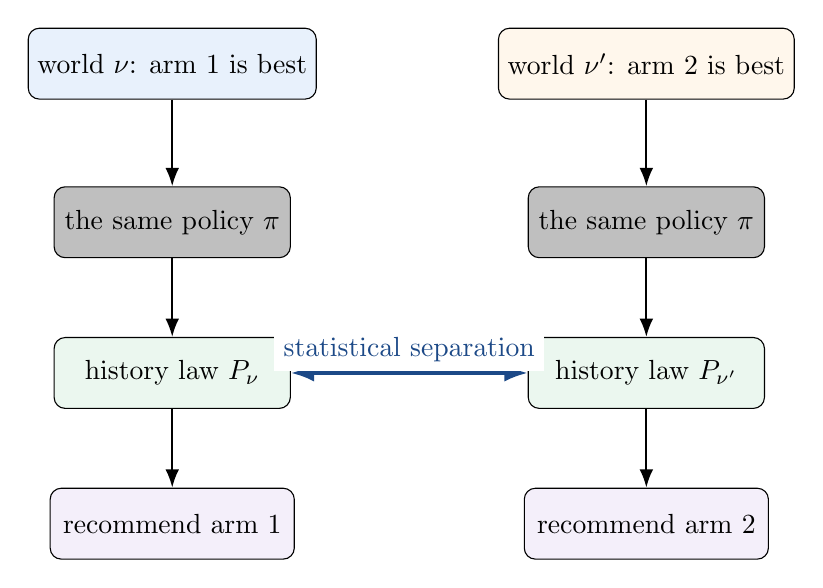
\begin{tikzpicture}[>=Latex,node distance=0.75cm]
\node[draw,rounded corners,fill=lightblue,minimum width=3.2cm,minimum height=0.9cm] (nu) {world $\nu$: arm 1 is best};
\node[draw,rounded corners,fill=lightorange,minimum width=3.2cm,minimum height=0.9cm,right=2.3cm of nu] (nup) {world $\nu'$: arm 2 is best};
\node[draw,rounded corners,fill=lightgray,minimum width=3.0cm,minimum height=0.9cm,below=1.1cm of nu] (p1) {the same policy $\pi$};
\node[draw,rounded corners,fill=lightgray,minimum width=3.0cm,minimum height=0.9cm,below=1.1cm of nup] (p2) {the same policy $\pi$};
\node[draw,rounded corners,fill=softgreen,minimum width=3.0cm,minimum height=0.9cm,below=1.0cm of p1] (h1) {history law $P_{\nu}$};
\node[draw,rounded corners,fill=softgreen,minimum width=3.0cm,minimum height=0.9cm,below=1.0cm of p2] (h2) {history law $P_{\nu'}$};
\node[draw,rounded corners,fill=softpurple,minimum width=3.1cm,minimum height=0.9cm,below=1.0cm of h1] (d1) {recommend arm 1};
\node[draw,rounded corners,fill=softpurple,minimum width=3.1cm,minimum height=0.9cm,below=1.0cm of h2] (d2) {recommend arm 2};
\draw[->,thick] (nu) -- (p1);
\draw[->,thick] (nup) -- (p2);
\draw[->,thick] (p1) -- (h1);
\draw[->,thick] (p2) -- (h2);
\draw[->,thick] (h1) -- (d1);
\draw[->,thick] (h2) -- (d2);
\draw[<->,very thick,mainblue] (h1) -- node[above,fill=white] {statistical separation} (h2);
\end{tikzpicture}
\caption{A lower bound compares the same algorithm under two environments that require different answers.}
\end{figure}

The proof strategy has three moving parts:

\begin{enumerate}
\item construct an alternative environment that changes the correct answer;
\item measure how much statistical evidence each observation supplies against that alternative;
\item show that reliable behavior in the two environments requires a minimum amount of total evidence.
\end{enumerate}

The first step is model design. The second is information accounting. The third is hypothesis testing.

\begin{keyidea}
A lower bound does not argue that an algorithm is clumsy. It argues that two worlds are too similar for \emph{any} algorithm to separate without paying for information.
\end{keyidea}

\chapter{One Coin, Two Possible Biases}

We begin without bandits. Suppose a coin has bias either $p$ or $q$, where $p\neq q$. Let
\[
P=\Ber(p),
\qquad
Q=\Ber(q).
\]
One toss produces $X\in\{0,1\}$.

If $X=1$, the probability of the observation is $p$ under $P$ and $q$ under $Q$. If $X=0$, the probabilities are $1-p$ and $1-q$. The likelihood ratio is therefore
\[
\frac{P(X)}{Q(X)}
=
\begin{cases}
\dfrac{p}{q}, & X=1,\\[0.8em]
\dfrac{1-p}{1-q}, & X=0.
\end{cases}
\]
Its logarithm can be written without cases:
\begin{equation}
\ell(X)
=
X\log\frac{p}{q}
+(1-X)\log\frac{1-p}{1-q}.
\label{eq:one-step-llr}
\end{equation}

A positive value favors $P$; a negative value favors $Q$.

\section{Evidence from several observations adds}

For independent observations $X_1,\ldots,X_n$,
\begin{align*}
\frac{P^n(X_1,\ldots,X_n)}{Q^n(X_1,\ldots,X_n)}
&=
\prod_{i=1}^{n}\frac{P(X_i)}{Q(X_i)},\\
L_n
:=
\log\frac{P^n(X_1,\ldots,X_n)}{Q^n(X_1,\ldots,X_n)}
&=
\sum_{i=1}^{n}\ell(X_i).
\end{align*}

The log-likelihood ratio is a ledger. Every observation adds one entry.

Under $P$, the expected entry is
\begin{align*}
\E_P[\ell(X)]
&=
\E_P\left[
X\log\frac{p}{q}
+(1-X)\log\frac{1-p}{1-q}
\right]\\
&=
\E_P[X]\log\frac{p}{q}
+\E_P[1-X]\log\frac{1-p}{1-q}\\
&=
p\log\frac{p}{q}
+(1-p)\log\frac{1-p}{1-q}\\
&=
\kl(p,q).
\end{align*}
Hence
\begin{equation}
\boxed{
\E_P[L_n]=n\,\kl(p,q).
}
\label{eq:iid-evidence-drift}
\end{equation}

KL divergence is not merely a distance-like quantity. In this experiment it is the expected evidence supplied by one observation.

\begin{figure}[H]
\centering

\includegraphics[width=0.82\textwidth]{assets/change-of-measure/evidence_paths.pdf}
\caption{Eight evidence paths under $P=\Ber(0.55)$ against $Q=\Ber(0.45)$. Individual paths wander, while the expected drift is $t\kl(0.55,0.45)$.}
\end{figure}

Some paths can favor the wrong model for a long time. That is not a defect in the calculation. It is the reason a lower bound exists. Evidence arrives with noise even when its average direction is correct.

\begin{thinkbox}
If $p$ and $q$ move closer, then $\kl(p,q)$ shrinks. The expected evidence per toss shrinks with it. A hard alternative is therefore not a wildly different world; it is a nearby world that changes the answer.
\end{thinkbox}

\chapter{Changing Measure, Without Mystery}

Let $P$ and $Q$ be two probability laws with densities $p$ and $q$ on the same sample space. Define
\[
L(x)=\log\frac{p(x)}{q(x)}.
\]
Then
\[
q(x)=p(x)e^{-L(x)}.
\]
For any event $E$,
\begin{align*}
Q(E)
&=\int_E q(x)\,\dd x\\
&=\int_E p(x)e^{-L(x)}\,\dd x\\
&=\E_P\left[\one_E e^{-L}\right].
\end{align*}
Thus
\begin{equation}
\boxed{
Q(E)=\E_P\left[\one_E e^{-L}\right].
}
\label{eq:change-measure-event}
\end{equation}

This is the change-of-measure identity. It says that a probability in the $Q$-world can be computed by averaging in the $P$-world, provided each outcome is reweighted by how much more or less plausible it is under $Q$.

There is no algorithm in this identity. It is a statement about two probability laws. Bandit lower bounds become possible when we apply it to the law of an entire adaptive history.

\section{Compressing the whole experiment to one event}

Suppose the final decision is summarized by an event $E$. Let
\[
\alpha=P(E),
\qquad
\beta=Q(E).
\]
The entire observation may be complicated, but the event records only one bit: did $E$ occur?

Information cannot increase when data are compressed. In this binary case,
\begin{equation}
\boxed{
\KL(P\Vert Q)\geq \kl(\alpha,\beta).
}
\label{eq:binary-data-processing}
\end{equation}

We now derive it directly.

On the event $E$, write $P_E$ and $Q_E$ for the conditional laws. Then
\[
P(\dd x)=\alpha P_E(\dd x),
\qquad
Q(\dd x)=\beta Q_E(\dd x),
\qquad x\in E.
\]
Therefore, on $E$,
\[
\frac{\dd P}{\dd Q}
=
\frac{\alpha}{\beta}
\frac{\dd P_E}{\dd Q_E}.
\]
The contribution of $E$ to KL is
\begin{align*}
\int_E \log\frac{\dd P}{\dd Q}\,\dd P
&=
\alpha\int_E
\log\left(
\frac{\alpha}{\beta}
\frac{\dd P_E}{\dd Q_E}
\right)\dd P_E\\
&=
\alpha\log\frac{\alpha}{\beta}
+
\alpha\KL(P_E\Vert Q_E).
\end{align*}
The same calculation on $E^c$ gives
\[
(1-\alpha)\log\frac{1-\alpha}{1-\beta}
+
(1-\alpha)\KL(P_{E^c}\Vert Q_{E^c}).
\]
Adding both pieces,
\begin{align*}
\KL(P\Vert Q)
&=
\alpha\log\frac{\alpha}{\beta}
+(1-\alpha)\log\frac{1-\alpha}{1-\beta}\\
&\quad
+
\alpha\KL(P_E\Vert Q_E)
+(1-\alpha)\KL(P_{E^c}\Vert Q_{E^c})\\
&\geq
\alpha\log\frac{\alpha}{\beta}
+(1-\alpha)\log\frac{1-\alpha}{1-\beta}\\
&=
\kl(\alpha,\beta).
\end{align*}
The inequality uses only the nonnegativity of KL divergence.

\begin{keyidea}
A lower-bound proof does not need to understand every feature of the final history. It can compress the history to the one event on which the two worlds must disagree.
\end{keyidea}

\section{A useful testing inequality}

Another common form is the Bretagnolle--Huber inequality. For every event $E$,
\begin{equation}
\boxed{
P(E)+Q(E^c)
\geq
\frac{1}{2}\exp\{-\KL(P\Vert Q)\}.
}
\label{eq:bh}
\end{equation}

Interpret $E$ as the decision ``choose $Q$.'' Then $P(E)$ is an error under $P$, while $Q(E^c)$ is an error under $Q$. Equation \eqref{eq:bh} says that the two errors cannot both be tiny unless the two laws have accumulated substantial KL divergence.

The complete proof is given in Appendix~\ref{app:bh-proof}. For now, the important shape is
\[
\text{testing error}
\gtrsim
e^{-\text{information}}.
\]

\begin{figure}[H]
\centering

\includegraphics[width=0.82\textwidth]{assets/change-of-measure/testing_error_bound.pdf}
\caption{The exact error of the optimal likelihood-ratio test and the Bretagnolle--Huber lower bound for $\Ber(0.4)$ versus $\Ber(0.6)$. The bound is not exact, but it captures the unavoidable exponential scale.}
\end{figure}

The bound is deliberately simple and therefore not always numerically tight. Its value is portability: the same inequality can be attached to an adaptive history, a stopping rule, or a recommendation event without redesigning the test from scratch.

\chapter{The Law of an Adaptive Bandit History}

Return to a $K$-armed bandit. Let
\[
\nu=(\nu_1,\ldots,\nu_K)
\]
be one environment and
\[
\nu'=(\nu'_1,\ldots,\nu'_K)
\]
be another. The policy is the same in both environments.

At round $t$, the policy chooses an arm $A_t$ from the past history
\[
H_{t-1}=(A_1,X_1,\ldots,A_{t-1},X_{t-1}).
\]
Write
\[
\pi_t(a\mid h_{t-1})
\]
for the probability that the policy chooses arm $a$ after history $h_{t-1}$. If arm $a$ is chosen, its reward density is $p_a$ under $\nu$ and $p'_a$ under $\nu'$.

For a realized history
\[
h_T=(a_1,x_1,\ldots,a_T,x_T),
\]
the density under $\nu$ factors as
\begin{equation}
P_\nu(h_T)
=
\prod_{t=1}^{T}
\pi_t(a_t\mid h_{t-1})p_{a_t}(x_t).
\label{eq:history-factorization-nu}
\end{equation}
Under $\nu'$,
\begin{equation}
P_{\nu'}(h_T)
=
\prod_{t=1}^{T}
\pi_t(a_t\mid h_{t-1})p'_{a_t}(x_t).
\label{eq:history-factorization-nup}
\end{equation}

\section{The policy terms cancel}

Divide \eqref{eq:history-factorization-nu} by \eqref{eq:history-factorization-nup}:
\begin{align*}
\frac{P_\nu(h_T)}{P_{\nu'}(h_T)}
&=
\frac{\prod_{t=1}^{T}\pi_t(a_t\mid h_{t-1})p_{a_t}(x_t)}
{\prod_{t=1}^{T}\pi_t(a_t\mid h_{t-1})p'_{a_t}(x_t)}\\
&=
\prod_{t=1}^{T}\frac{p_{a_t}(x_t)}{p'_{a_t}(x_t)}.
\end{align*}
Therefore the history log-likelihood ratio is
\begin{equation}
L_T
=
\sum_{t=1}^{T}
\log\frac{p_{A_t}(X_t)}{p'_{A_t}(X_t)}.
\label{eq:bandit-llr}
\end{equation}

This cancellation is the central algebraic fact. The policy may be adaptive, randomized, and highly nonlinear. None of those policy probabilities appears in the final likelihood ratio, because the same decision rule is used in both worlds.

\begin{figure}[H]
\centering
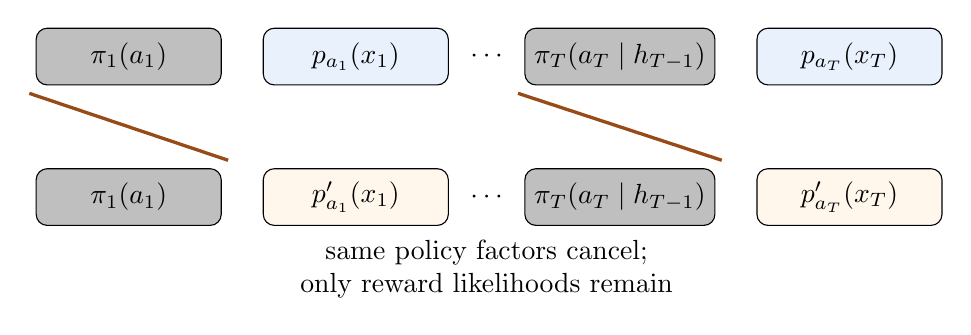
\begin{tikzpicture}[>=Latex,node distance=0.52cm]
\node[draw,rounded corners,fill=lightgray,minimum width=2.35cm,minimum height=0.72cm] (pi1) {$\pi_1(a_1)$};
\node[draw,rounded corners,fill=lightblue,minimum width=2.35cm,minimum height=0.72cm,right=of pi1] (p1) {$p_{a_1}(x_1)$};
\node[right=0.15cm of p1] (dots1) {$\cdots$};
\node[draw,rounded corners,fill=lightgray,minimum width=2.35cm,minimum height=0.72cm,right=0.15cm of dots1] (pit) {$\pi_T(a_T\mid h_{T-1})$};
\node[draw,rounded corners,fill=lightblue,minimum width=2.35cm,minimum height=0.72cm,right=of pit] (pt) {$p_{a_T}(x_T)$};

\node[draw,rounded corners,fill=lightgray,minimum width=2.35cm,minimum height=0.72cm,below=1.05cm of pi1] (qpi1) {$\pi_1(a_1)$};
\node[draw,rounded corners,fill=lightorange,minimum width=2.35cm,minimum height=0.72cm,right=of qpi1] (q1) {$p'_{a_1}(x_1)$};
\node[right=0.15cm of q1] (dots2) {$\cdots$};
\node[draw,rounded corners,fill=lightgray,minimum width=2.35cm,minimum height=0.72cm,right=0.15cm of dots2] (qpit) {$\pi_T(a_T\mid h_{T-1})$};
\node[draw,rounded corners,fill=lightorange,minimum width=2.35cm,minimum height=0.72cm,right=of qpit] (qt) {$p'_{a_T}(x_T)$};

\draw[very thick,deeporange] ($(pi1.south west)+(-0.08,-0.10)$) -- ($(qpi1.north east)+(0.08,0.10)$);
\draw[very thick,deeporange] ($(pit.south west)+(-0.08,-0.10)$) -- ($(qpit.north east)+(0.08,0.10)$);
\node[below=0.22cm of dots2,align=center] {same policy factors cancel;\\only reward likelihoods remain};
\end{tikzpicture}
\caption{The learner's adaptivity changes which reward factors appear, but not the likelihood-ratio algebra.}
\end{figure}

\section{Expected evidence equals pulls times armwise KL}

Take expectations under $\nu$. From \eqref{eq:bandit-llr},
\begin{align*}
\E_\nu[L_T]
&=
\sum_{t=1}^{T}
\E_\nu\left[
\log\frac{p_{A_t}(X_t)}{p'_{A_t}(X_t)}
\right].
\end{align*}
Condition on the selected arm. If $A_t=a$, then $X_t\sim\nu_a$ under $\nu$, and therefore
\begin{align*}
\E_\nu\left[
\left.
\log\frac{p_{A_t}(X_t)}{p'_{A_t}(X_t)}
\right|A_t=a, H_{t-1}
\right]
&=
\int p_a(x)\log\frac{p_a(x)}{p'_a(x)}\,\dd x\\
&=
\KL(\nu_a\Vert\nu'_a).
\end{align*}
Hence
\begin{align*}
\E_\nu[L_T]
&=
\sum_{t=1}^{T}
\E_\nu\left[\KL(\nu_{A_t}\Vert\nu'_{A_t})\right]\\
&=
\sum_{t=1}^{T}
\sum_{a=1}^{K}
\Pbb_\nu(A_t=a)\KL(\nu_a\Vert\nu'_a)\\
&=
\sum_{a=1}^{K}
\E_\nu\left[
\sum_{t=1}^{T}\one\{A_t=a\}
\right]
\KL(\nu_a\Vert\nu'_a).
\end{align*}
Define the number of pulls
\[
N_a(T)=\sum_{t=1}^{T}\one\{A_t=a\}.
\]
Then
\begin{equation}
\boxed{
\KL(P_\nu^T\Vert P_{\nu'}^T)
=
\E_\nu[L_T]
=
\sum_{a=1}^{K}
\E_\nu[N_a(T)]\KL(\nu_a\Vert\nu'_a).
}
\label{eq:divergence-decomposition}
\end{equation}

This is often called the divergence decomposition. It turns a complicated adaptive experiment into a simple information ledger:

\begin{center}
\emph{expected pulls of arm $a$}\quad$\times$\quad\emph{information supplied by one pull of arm $a$}.
\end{center}

\begin{keyidea}
Adaptivity changes the random pull counts. It does not create information from nowhere. Every unit of KL must still be paid for by observations from arms on which the two environments differ.
\end{keyidea}

\section{A numerical audit of the identity}

The supplied code runs UCB under
\[
\nu=(\Ber(0.62),\Ber(0.50))
\]
and compares it with the alternative
\[
\nu'=(\Ber(0.62),\Ber(0.68)).
\]
Only arm 2 changes. For each simulated history we compute the realized log-likelihood ratio and compare its average with
\[
\E_\nu[N_2(T)]\kl(0.50,0.68).
\]

\begin{figure}[H]
\centering

\includegraphics[width=0.82\textwidth]{assets/change-of-measure/adaptive_information_identity.pdf}
\caption{The empirical mean log-likelihood ratio matches the pull-count information ledger, even though the sampling rule is adaptive.}
\end{figure}

\begin{table}[H]
\centering
\caption{Adaptive information accounting under UCB, based on 12,000 replications.}
\begin{tabular}{rrrr}
\toprule
Horizon & $\E[N_2(T)]$ & empirical $\E[L_T]$ & $\E[N_2(T)]\kl(0.50,0.68)$ \\
\midrule
100  & 37.05  & 2.581 & 2.572 \\
400  & 114.50 & 7.997 & 7.946 \\
800  & 187.81 & 13.040 & 13.034 \\
1200 & 244.16 & 16.966 & 16.945 \\
\bottomrule
\end{tabular}
\end{table}

The code performing the essential update is short:

\begin{codeblock}{Python}
means = sums / counts
bonus = np.sqrt(2.0 * np.log(t + 1.0) / counts)
actions = np.argmax(means + bonus, axis=1)

arm_means = true_means[actions]
alt_means = alternative_means[actions]
rewards = rng.binomial(1, arm_means).astype(float)

counts[indices, actions] += 1
sums[indices, actions] += rewards

total_llr += (
    rewards * np.log(arm_means / alt_means)
    + (1.0 - rewards)
      * np.log((1.0 - arm_means) / (1.0 - alt_means))
)
\end{codeblock}

\chapter{Stopping When the Evidence Is Enough}

Many bandit algorithms do not stop at a fixed horizon. They stop when the data appear decisive. Let $\tau$ be such a stopping time, and let $\calF_\tau$ contain everything known when the algorithm stops.

The stopped log-likelihood ratio is
\[
L_\tau
=
\sum_{t=1}^{\tau}
\log\frac{p_{A_t}(X_t)}{p'_{A_t}(X_t)}.
\]
Under the usual integrability conditions, the same information ledger holds:
\begin{equation}
\E_\nu[L_\tau]
=
\sum_{a=1}^{K}
\E_\nu[N_a(\tau)]\KL(\nu_a\Vert\nu'_a).
\label{eq:stopped-ledger}
\end{equation}

Now take any event $E\in\calF_\tau$. It could be the event that the algorithm recommends arm 1, eliminates arm 4, or stops before a given time. Applying binary data processing to the stopped history gives
\[
\E_\nu[L_\tau]
\geq
\kl\bigl(\Pbb_\nu(E),\Pbb_{\nu'}(E)\bigr).
\]
Combining with \eqref{eq:stopped-ledger} yields the fundamental bandit change-of-measure inequality.

\begin{resultbox}[title=Bandit transportation inequality]
For two bandit environments $\nu$ and $\nu'$, an almost surely finite stopping time $\tau$, and any event $E\in\calF_\tau$,
\begin{equation}
\boxed{
\sum_{a=1}^{K}
\E_\nu[N_a(\tau)]\KL(\nu_a\Vert\nu'_a)
\geq
\kl\bigl(\Pbb_\nu(E),\Pbb_{\nu'}(E)\bigr).
}
\label{eq:transportation}
\end{equation}
\end{resultbox}

The word ``transportation'' is helpful. The left side measures how much information the algorithm transports from observations into its history. The right side measures how far apart the algorithm's behavior must be in the two worlds.

\section{The proof in three transparent steps}

\textbf{Step 1: the stopped change-of-measure identity.}
For $E\in\calF_\tau$,
\[
\Pbb_{\nu'}(E)
=
\E_\nu\left[\one_E e^{-L_\tau}\right].
\]

\textbf{Step 2: compress the stopped history to $E$.}
The laws of the whole stopped history satisfy
\[
\KL(P_\nu^{H_\tau}\Vert P_{\nu'}^{H_\tau})
\geq
\kl\bigl(\Pbb_\nu(E),\Pbb_{\nu'}(E)\bigr).
\]
Since the log density ratio of the stopped histories is $L_\tau$,
\[
\KL(P_\nu^{H_\tau}\Vert P_{\nu'}^{H_\tau})
=
\E_\nu[L_\tau].
\]

\textbf{Step 3: expand the expected evidence arm by arm.}
Write the observations from arm $a$ in their order of appearance as
\[
Y_{a,1},Y_{a,2},\ldots.
\]
Then
\[
L_\tau
=
\sum_{a=1}^{K}
\sum_{s=1}^{N_a(\tau)}
\log\frac{p_a(Y_{a,s})}{p'_a(Y_{a,s})}.
\]
The expected increment from arm $a$ is
\[
\E_\nu\left[
\log\frac{p_a(Y_{a,s})}{p'_a(Y_{a,s})}
\right]
=
\KL(\nu_a\Vert\nu'_a).
\]
Wald's identity therefore gives
\[
\E_\nu[L_\tau]
=
\sum_{a=1}^{K}
\E_\nu[N_a(\tau)]\KL(\nu_a\Vert\nu'_a).
\]
Putting the three steps together proves \eqref{eq:transportation}.

\begin{patternbox}
A change-of-measure lower bound usually has the same skeleton:
\[
\text{sample allocation}
\longrightarrow
\text{KL information}
\longrightarrow
\text{separation of a decision event}.
\]
The creativity lies mainly in choosing the alternative environment and the event.
\end{patternbox}

\chapter{The Simplest Sample-Complexity Lower Bound}

Return once more to the two-coin problem. Suppose a decision rule observes $n$ tosses and must identify whether the coin is $P=\Ber(p)$ or $Q=\Ber(q)$. Let
\[
E=\{\text{the rule declares }P\}.
\]
Assume the rule has error at most $\delta$ in both worlds:
\[
P^n(E)\geq 1-\delta,
\qquad
Q^n(E)\leq\delta.
\]
By \eqref{eq:binary-data-processing},
\begin{align*}
\KL(P^n\Vert Q^n)
&\geq
\kl\bigl(P^n(E),Q^n(E)\bigr)\\
&\geq
\kl(1-\delta,\delta).
\end{align*}
Independence gives
\[
\KL(P^n\Vert Q^n)=n\KL(P\Vert Q)=n\kl(p,q).
\]
Therefore
\begin{equation}
\boxed{
 n
 \geq
 \frac{\kl(1-\delta,\delta)}{\kl(p,q)}.
}
\label{eq:coin-lower-bound}
\end{equation}

Every part has an interpretation:

\[
\underbrace{n}_{\text{number of observations}}
\times
\underbrace{\kl(p,q)}_{\text{evidence per observation}}
\geq
\underbrace{\kl(1-\delta,\delta)}_{\text{evidence demanded by reliability}}.
\]

For $p=0.55$, $q=0.45$, and $\delta=0.05$,
\[
\kl(0.55,0.45)\approx0.02007,
\qquad
\kl(0.95,0.05)\approx2.650.
\]
Thus
\[
n\geq\frac{2.650}{0.02007}\approx132.1.
\]
A rule that promises five-percent error in both directions needs at least about 133 tosses according to this information bound.

As $\delta\downarrow0$,
\[
\kl(1-\delta,\delta)
=(1-2\delta)\log\frac{1-\delta}{\delta}
\sim
\log\frac{1}{\delta}.
\]
So the familiar logarithm in fixed-confidence sample complexity is not an artifact of one algorithm. It is the amount of evidence required to drive an error probability down to $\delta$.

\chapter{Best-Arm Identification: Make the Answer Change}

Consider a bandit environment $\nu$ with a unique best arm
\[
a^*(\nu)=\argmax_a \mu_a.
\]
A fixed-confidence algorithm stops at $\tau$ and recommends $\widehat a$. It is $\delta$-correct if
\[
\Pbb_\nu(\widehat a=a^*(\nu))\geq1-\delta
\]
for every environment in the model class.

Fix the true environment $\nu$. Now choose an alternative $\lambda$ whose best arm is different:
\[
a^*(\lambda)\neq a^*(\nu).
\]
Define
\[
E=\{\widehat a=a^*(\nu)\}.
\]
Correctness in the true world gives
\[
\Pbb_\nu(E)\geq1-\delta.
\]
Correctness in the alternative world gives
\[
\Pbb_\lambda(E)\leq\delta,
\]
because the arm recommended on $E$ is wrong under $\lambda$.

Insert this event into the transportation inequality:
\begin{equation}
\boxed{
\sum_{a=1}^{K}
\E_\nu[N_a(\tau)]\KL(\nu_a\Vert\lambda_a)
\geq
\kl(1-\delta,\delta).
}
\label{eq:bai-one-alternative}
\end{equation}

This inequality holds for \emph{every} alternative that changes the best arm.

\section{A first, deliberately simple alternative}

Suppose there are two Bernoulli arms with
\[
\mu_1>\mu_2.
\]
Keep arm 1 unchanged and raise arm 2 to a mean $\lambda_2>\mu_1$. Then only arm 2 differs, and \eqref{eq:bai-one-alternative} becomes
\[
\E_\nu[N_2(\tau)]\kl(\mu_2,\lambda_2)
\geq
\kl(1-\delta,\delta).
\]
Hence
\begin{equation}
\E_\nu[N_2(\tau)]
\geq
\frac{\kl(1-\delta,\delta)}{\kl(\mu_2,\lambda_2)}.
\label{eq:single-arm-bai-bound}
\end{equation}

Let $\lambda_2$ approach $\mu_1$ from above. The alternative becomes as close as possible while still changing the best arm, yielding
\[
\E_\nu[N_2(\tau)]
\gtrsim
\frac{\kl(1-\delta,\delta)}{\kl(\mu_2,\mu_1)}.
\]

This already explains why a suboptimal arm cannot simply be ignored. If the learner rarely samples arm 2, it cannot rule out the nearby world in which arm 2 is actually best.

\begin{thinkbox}
Why not raise arm 2 to $0.99$? Because that alternative is easy to distinguish. Its KL divergence is large, so the resulting lower bound is weak. Lower bounds become strong by finding the \emph{closest answer-changing alternative}.
\end{thinkbox}

\section{The allocation game}

Let
\[
\Alt(\nu)
=
\{\lambda:a^*(\lambda)\neq a^*(\nu)\}
\]
be the set of answer-changing alternatives. Define the expected allocation proportions
\[
w_a
=
\frac{\E_\nu[N_a(\tau)]}{\E_\nu[\tau]},
\qquad
\sum_{a=1}^{K}w_a=1.
\]
Then \eqref{eq:bai-one-alternative} can be written
\[
\E_\nu[\tau]
\sum_{a=1}^{K}w_a\KL(\nu_a\Vert\lambda_a)
\geq
\kl(1-\delta,\delta).
\]
Because this must hold for every $\lambda\in\Alt(\nu)$,
\[
\E_\nu[\tau]
\inf_{\lambda\in\Alt(\nu)}
\sum_{a=1}^{K}w_a\KL(\nu_a\Vert\lambda_a)
\geq
\kl(1-\delta,\delta).
\]
Thus
\begin{equation}
\E_\nu[\tau]
\geq
\frac{\kl(1-\delta,\delta)}
{\displaystyle
\inf_{\lambda\in\Alt(\nu)}
\sum_{a=1}^{K}w_a\KL(\nu_a\Vert\lambda_a)}.
\label{eq:allocation-specific-lb}
\end{equation}

The algorithm chooses $w$. The lower-bound argument then chooses the hardest alternative against that allocation. This leads to the characteristic information value
\begin{equation}
\boxed{
\frac{1}{T^*(\nu)}
=
\sup_{w\in\Delta_K}
\inf_{\lambda\in\Alt(\nu)}
\sum_{a=1}^{K}w_a\KL(\nu_a\Vert\lambda_a),
}
\label{eq:t-star}
\end{equation}
where
\[
\Delta_K
=
\left\{w\in[0,1]^K:\sum_{a=1}^{K}w_a=1\right\}.
\]
Consequently,
\begin{equation}
\E_\nu[\tau]
\geq
T^*(\nu)\,\kl(1-\delta,\delta).
\label{eq:tstar-lb}
\end{equation}

\begin{researchbox}
Equation \eqref{eq:t-star} is not only a lower bound. It is an algorithm-design target. Track-and-Stop and later best-arm identification methods attempt to learn and track the allocation that maximizes the worst-case information rate. The same information-allocation viewpoint also underlies modern batched BAI and regret-aware BAI, including research directions developed by Tianyuan Jin and collaborators.
\end{researchbox}

\chapter{Two Gaussian Arms: Solve the Lower-Bound Game Completely}

Consider two Gaussian arms with known common variance $\sigma^2$:
\[
\nu_1=\Normal(\mu_1,\sigma^2),
\qquad
\nu_2=\Normal(\mu_2,\sigma^2),
\qquad
\mu_1>\mu_2.
\]
Let
\[
\Delta=\mu_1-\mu_2>0.
\]
Assign a fraction $w$ of samples to arm 1 and $1-w$ to arm 2.

For an alternative mean vector $(\lambda_1,\lambda_2)$, Gaussian KL gives
\[
\KL\bigl(\Normal(\mu_a,\sigma^2)\Vert\Normal(\lambda_a,\sigma^2)\bigr)
=
\frac{(\mu_a-\lambda_a)^2}{2\sigma^2}.
\]
The information rate is therefore
\begin{equation}
I_w(\lambda_1,\lambda_2)
=
\frac{w(\mu_1-\lambda_1)^2
+(1-w)(\mu_2-\lambda_2)^2}{2\sigma^2}.
\label{eq:gaussian-rate}
\end{equation}

The alternative must make arm 2 at least as good as arm 1:
\[
\lambda_1\leq\lambda_2.
\]
The closest point in this half-space lies on the boundary
\[
\lambda_1=\lambda_2=m.
\]
Thus we minimize
\[
I_w(m)
=
\frac{w(\mu_1-m)^2+(1-w)(\mu_2-m)^2}{2\sigma^2}.
\]

\section{Step 1: find the hardest common mean}

Differentiate with respect to $m$:
\begin{align*}
\frac{\dd}{\dd m}
\left[
 w(\mu_1-m)^2+(1-w)(\mu_2-m)^2
\right]
&=
2w(m-\mu_1)+2(1-w)(m-\mu_2).
\end{align*}
Set this equal to zero:
\begin{align*}
0
&=
w(m-\mu_1)+(1-w)(m-\mu_2)\\
&=
m-w\mu_1-(1-w)\mu_2.
\end{align*}
Therefore
\begin{equation}
\boxed{
 m_w=w\mu_1+(1-w)\mu_2.
}
\label{eq:hardest-m}
\end{equation}

The hard alternative moves toward the arm receiving fewer samples. If arm 1 receives most of the budget, then its mean is well measured and the alternative moves close to $\mu_1$, leaving the poorly measured arm 2 to do most of the work.

\begin{figure}[H]
\centering

\includegraphics[width=0.82\textwidth]{assets/change-of-measure/gaussian_alternative_geometry.pdf}
\caption{For each allocation $w$, the hardest boundary alternative is the minimum of the corresponding quadratic information curve.}
\end{figure}

\section{Step 2: substitute the minimizer}

From \eqref{eq:hardest-m},
\begin{align*}
\mu_1-m_w
&=
\mu_1-w\mu_1-(1-w)\mu_2\\
&=
(1-w)(\mu_1-\mu_2)\\
&=
(1-w)\Delta,
\end{align*}
and
\begin{align*}
\mu_2-m_w
&=
\mu_2-w\mu_1-(1-w)\mu_2\\
&=
-w(\mu_1-\mu_2)\\
&=
-w\Delta.
\end{align*}
Therefore
\begin{align*}
\inf_{\lambda_1\leq\lambda_2}I_w(\lambda_1,\lambda_2)
&=
\frac{w(1-w)^2\Delta^2+(1-w)w^2\Delta^2}{2\sigma^2}\\
&=
\frac{w(1-w)\bigl((1-w)+w\bigr)\Delta^2}{2\sigma^2}\\
&=
\frac{w(1-w)\Delta^2}{2\sigma^2}.
\end{align*}

\section{Step 3: choose the best allocation}

Since
\[
w(1-w)
=
\frac14-\left(w-\frac12\right)^2,
\]
the maximum occurs at
\[
w^*=\frac12.
\]
The optimal information rate is
\begin{equation}
\frac{1}{T^*(\nu)}
=
\frac{\Delta^2}{8\sigma^2}.
\label{eq:gaussian-tstar-rate}
\end{equation}
Hence
\begin{equation}
\boxed{
\E_\nu[\tau]
\geq
\frac{8\sigma^2}{\Delta^2}
\kl(1-\delta,\delta).
}
\label{eq:gaussian-bai-lb}
\end{equation}

\begin{figure}[H]
\centering

\includegraphics[width=0.82\textwidth]{assets/change-of-measure/gaussian_information_rate.pdf}
\caption{The worst-case information rate is maximized by equal allocation in the symmetric two-Gaussian problem.}
\end{figure}

This conclusion is easy to say after the calculation: both sample means enter the comparison, so making one estimate precise while leaving the other noisy is wasteful. The lower-bound game turns that intuition into an exact constant.

\section{The same allocation appears in the actual error}

With a fixed total budget $n$, let
\[
n_1=wn,
\qquad
n_2=(1-w)n.
\]
The sample-mean difference satisfies
\[
\widehat\mu_1-\widehat\mu_2
\sim
\Normal\left(
\Delta,
\sigma^2\left(\frac1{n_1}+\frac1{n_2}\right)
\right).
\]
If the learner recommends the larger sample mean, then
\begin{align*}
\Pbb(\text{error})
&=
\Pbb(\widehat\mu_1-\widehat\mu_2\leq0)\\
&=
\Phi\left(
-\frac{\Delta}
{\sigma\sqrt{1/n_1+1/n_2}}
\right).
\end{align*}
The denominator is minimized at $n_1=n_2$. Thus the finite-sample testing calculation and the information lower bound select the same allocation.

\begin{figure}[H]
\centering

\includegraphics[width=0.82\textwidth]{assets/change-of-measure/gaussian_allocation_error.pdf}
\caption{For $n=400$, $(\mu_1,\mu_2)=(0.2,0)$, and $\sigma=1$, both exact calculation and Monte Carlo show that equal allocation minimizes the recommendation error.}
\end{figure}

\begin{table}[H]
\centering
\caption{Selected Gaussian allocation results.}
\begin{tabular}{rrr}
\toprule
Fraction $w$ on arm 1 & exact error probability & information rate \\
\midrule
0.10 & 0.1151 & 0.00180 \\
0.30 & 0.0334 & 0.00420 \\
0.50 & 0.0228 & 0.00500 \\
0.70 & 0.0334 & 0.00420 \\
0.90 & 0.1151 & 0.00180 \\
\bottomrule
\end{tabular}
\end{table}

\begin{codeblock}{Python}
n1 = max(1, int(round(total_budget * weight)))
n2 = total_budget - n1

mean1 = mu1 + sigma / np.sqrt(n1) * rng.standard_normal(replications)
mean2 = mu2 + sigma / np.sqrt(n2) * rng.standard_normal(replications)
empirical_error = np.mean(mean1 <= mean2)

standard_error = sigma * np.sqrt(1.0 / n1 + 1.0 / n2)
exact_error = norm.cdf(-(mu1 - mu2) / standard_error)
\end{codeblock}

\chapter{A Glimpse of the Lai--Robbins Regret Lower Bound}

The same argument also explains why logarithmic exploration is unavoidable in regret minimization.

Suppose arm $a$ is suboptimal under $\nu$:
\[
\mu_a<\mu^*.
\]
Construct an alternative $\nu'$ that changes only arm $a$, making it slightly better than $\mu^*$. If the algorithm almost never samples arm $a$ under $\nu$, then the histories under $\nu$ and $\nu'$ remain too similar. But a good policy must behave differently:

\begin{itemize}
\item under $\nu$, it should pull arm $a$ rarely;
\item under $\nu'$, it should pull arm $a$ almost all the time.
\end{itemize}

Choose an event such as
\[
E_T=\left\{N_a(T)<\frac{T}{2}\right\}.
\]
For a sufficiently efficient policy,
\[
\Pbb_\nu(E_T)\to1,
\qquad
\Pbb_{\nu'}(E_T)\to0.
\]
The transportation inequality gives
\begin{equation}
\E_\nu[N_a(T)]\KL(\nu_a\Vert\nu'_a)
\geq
\kl\bigl(\Pbb_\nu(E_T),\Pbb_{\nu'}(E_T)\bigr).
\label{eq:regret-preview}
\end{equation}
Under the consistency conditions used by Lai and Robbins, the right side grows like $\log T$. Moving $\nu'_a$ down toward the boundary where its mean equals $\mu^*$ yields
\begin{equation}
\liminf_{T\to\infty}
\frac{\E_\nu[N_a(T)]}{\log T}
\geq
\frac{1}{\KL(\nu_a\Vert\nu^*)}.
\label{eq:lai-robbins-pull-preview}
\end{equation}
Multiplying by the regret gap $\Delta_a=\mu^*-\mu_a$ and summing gives the classical shape
\begin{equation}
\liminf_{T\to\infty}
\frac{R_T(\nu)}{\log T}
\geq
\sum_{a:\Delta_a>0}
\frac{\Delta_a}{\KL(\nu_a\Vert\nu^*)}.
\label{eq:lai-robbins-preview}
\end{equation}

This section is only the proof skeleton. The next chapter will state the consistency assumptions carefully, construct the event with the correct polynomial probabilities, and derive the full Lai--Robbins lower bound without hiding the asymptotic steps.

\begin{keyidea}
The logarithmic exploration rate is the price of ruling out a nearby world in which a currently suboptimal arm is actually optimal.
\end{keyidea}

\chapter{What the Experiments Are Checking}

The numerical work in this chapter serves as a proof audit rather than as evidence for the theorem.

\section{Evidence paths}

For $X_t\sim\Ber(p)$, the cumulative evidence against $q$ is
\[
L_t
=
\sum_{s=1}^{t}
\left[
X_s\log\frac{p}{q}
+(1-X_s)\log\frac{1-p}{1-q}
\right].
\]
The experiment checks that paths are noisy while their mean slope is $\kl(p,q)$.

\section{Testing error}

For each $n$, the script computes the exact sum of type-I and type-II errors of the equal-prior likelihood-ratio test between $\Ber(0.4)^n$ and $\Ber(0.6)^n$. It compares this with
\[
\frac12e^{-n\kl(0.4,0.6)}.
\]

\begin{table}[H]
\centering
\caption{Optimal testing error versus the Bretagnolle--Huber lower bound.}
\begin{tabular}{rrr}
\toprule
$n$ & exact sum of errors & lower bound \\
\midrule
10  & 0.5331 & 0.2222 \\
20  & 0.3722 & 0.0988 \\
40  & 0.2041 & 0.0195 \\
80  & 0.0716 & 0.000761 \\
160 & 0.0107 & $1.16\times10^{-6}$ \\
\bottomrule
\end{tabular}
\end{table}

The lower bound becomes loose in this example because it sacrifices constants for generality. It is still correct, and it preserves the central message that the error cannot decay independently of accumulated information.

\section{Adaptive information accounting}

The UCB experiment checks
\[
\E_\nu[L_T]
=
\sum_a\E_\nu[N_a(T)]\KL(\nu_a\Vert\nu'_a)
\]
under an adaptive policy. The near overlap of the two curves is a direct numerical check that the likelihood-ratio implementation, pull counts, and KL formula agree.

\section{Allocation and hard alternatives}

The Gaussian experiment checks two linked predictions:

\[
\text{hardest alternative for allocation }w
\quad\Longrightarrow\quad
m_w=w\mu_1+(1-w)\mu_2,
\]
and
\[
\text{best worst-case information rate}
\quad\Longrightarrow\quad
w^*=\frac12.
\]
The exact finite-sample error confirms the same symmetry.

\begin{thinkbox}
A simulation can reveal a coding error or a missing factor of two. It cannot prove a universal lower bound. The proof ranges over all algorithms and all admissible alternatives; a simulation samples only finitely many histories from one implementation.
\end{thinkbox}

\chapter{Common Mistakes in Change-of-Measure Proofs}

\section{Choosing an alternative that does not change the answer}

If $a^*(\lambda)=a^*(\nu)$, then the recommendation event need not have very different probabilities. The right side of \eqref{eq:transportation} may be small, and no useful lower bound follows.

\section{Choosing an alternative that is too far away}

A dramatic alternative has a large KL cost per observation. Since the lower bound divides by this cost, the result becomes weak. The right alternative usually sits near the decision boundary.

\section{Reversing the direction of KL}

The expected log-likelihood ratio under $\nu$ is
\[
\E_\nu\left[\log\frac{\dd P_\nu}{\dd P_{\nu'}}\right]
=
\KL(P_\nu\Vert P_{\nu'}),
\]
not the reverse divergence. The pull counts are also averaged under $\nu$. Both directions must match.

\section{Forgetting that counts are random}

In an adaptive bandit, $N_a(T)$ depends on previous rewards. The correct identity uses
\[
\E_\nu[N_a(T)]\KL(\nu_a\Vert\nu'_a),
\]
not a deterministic count inserted after the fact.

\section{Using an event unavailable at the stopping time}

The event $E$ must belong to $\calF_\tau$. A lower-bound proof cannot use future observations that the algorithm did not possess when it stopped.

\section{Proving correctness only in the true environment}

The argument needs the algorithm to be reliable in both $\nu$ and $\lambda$. This is why lower bounds assume uniform correctness over a model class. A procedure designed for one known instance could simply print the answer without observing anything.

\section{Stopping after one convenient alternative}

One alternative gives one constraint. A sharp lower bound minimizes over every answer-changing alternative and then optimizes the sampling allocation. The optimization is the theorem, not decorative notation.

\chapter{What to Carry Forward}

The chapter can be compressed to five equations.

For two laws,
\[
Q(E)=\E_P[\one_Ee^{-L}],
\qquad
L=\log\frac{\dd P}{\dd Q}.
\]

Compressing an experiment to an event cannot increase information:
\[
\KL(P\Vert Q)
\geq
\kl(P(E),Q(E)).
\]

For a fixed-horizon adaptive bandit,
\[
\KL(P_\nu^T\Vert P_{\nu'}^T)
=
\sum_a\E_\nu[N_a(T)]\KL(\nu_a\Vert\nu'_a).
\]

For a stopped experiment and $E\in\calF_\tau$,
\[
\sum_a\E_\nu[N_a(\tau)]\KL(\nu_a\Vert\nu'_a)
\geq
\kl(\Pbb_\nu(E),\Pbb_{\nu'}(E)).
\]

For fixed-confidence best-arm identification,
\[
\frac1{T^*(\nu)}
=
\sup_{w\in\Delta_K}
\inf_{\lambda\in\Alt(\nu)}
\sum_a w_a\KL(\nu_a\Vert\lambda_a).
\]

These equations express one idea in progressively richer settings:

\begin{center}
\emph{To behave differently in two nearby worlds, a learner must observe enough of the places where those worlds differ.}
\end{center}

\begin{figure}[H]
\centering
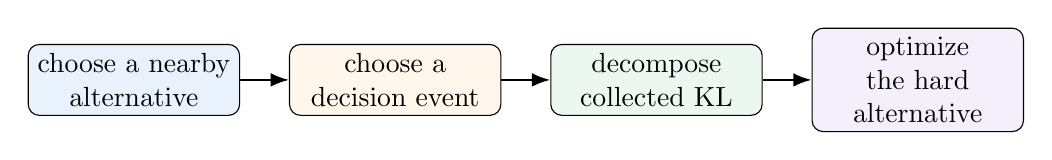
\begin{tikzpicture}[>=Latex,node distance=0.62cm]
\node[draw,rounded corners,fill=lightblue,text width=2.45cm,align=center,minimum height=0.82cm] (alt) {choose a nearby alternative};
\node[draw,rounded corners,fill=lightorange,text width=2.45cm,align=center,minimum height=0.82cm,right=of alt] (event) {choose a decision event};
\node[draw,rounded corners,fill=softgreen,text width=2.45cm,align=center,minimum height=0.82cm,right=of event] (info) {decompose collected KL};
\node[draw,rounded corners,fill=softpurple,text width=2.45cm,align=center,minimum height=0.82cm,right=of info] (opt) {optimize the hard alternative};
\draw[->,thick] (alt) -- (event);
\draw[->,thick] (event) -- (info);
\draw[->,thick] (info) -- (opt);
\end{tikzpicture}
\caption{The reusable research pattern behind many bandit lower bounds.}
\end{figure}

\appendix

\chapter*{Proof of the Bretagnolle--Huber Inequality}
\addcontentsline{toc}{chapter}{Proof of the Bretagnolle--Huber Inequality}
\label{app:bh-proof}

Let $p$ and $q$ be densities of $P$ and $Q$ with respect to a common measure. For any event $E$,
\begin{align*}
P(E)+Q(E^c)
&=
\int_E p+\int_{E^c}q\\
&\geq
\int \min\{p,q\}.
\end{align*}
Define the affinity
\[
\rho(P,Q)=\int\sqrt{pq}.
\]
By Cauchy--Schwarz,
\begin{align*}
\rho(P,Q)^2
&=
\left(
\int
\sqrt{\min\{p,q\}}
\sqrt{\max\{p,q\}}
\right)^2\\
&\leq
\left(\int\min\{p,q\}\right)
\left(\int\max\{p,q\}\right).
\end{align*}
Since
\[
\int\max\{p,q\}
=2-\int\min\{p,q\}
\leq2,
\]
we obtain
\begin{equation}
\int\min\{p,q\}
\geq
\frac{\rho(P,Q)^2}{2}.
\label{eq:min-affinity}
\end{equation}

Next relate affinity to KL. Under $P$,
\begin{align*}
\rho(P,Q)
&=
\int p\sqrt{\frac{q}{p}}\\
&=
\E_P\left[\sqrt{\frac{q}{p}}\right].
\end{align*}
Because $-\log$ is convex, Jensen's inequality gives
\begin{align*}
-\log\rho(P,Q)
&\leq
\E_P\left[
-\log\sqrt{\frac{q}{p}}
\right]\\
&=
\frac12\E_P\left[\log\frac{p}{q}\right]\\
&=
\frac12\KL(P\Vert Q).
\end{align*}
Therefore
\[
\rho(P,Q)
\geq
\exp\left\{-\frac12\KL(P\Vert Q)\right\}.
\]
Squaring and substituting into \eqref{eq:min-affinity},
\[
\int\min\{p,q\}
\geq
\frac12e^{-\KL(P\Vert Q)}.
\]
Finally,
\[
P(E)+Q(E^c)
\geq
\int\min\{p,q\}
\geq
\frac12e^{-\KL(P\Vert Q)}.
\]

\chapter*{A Direct Jensen Proof of Event Compression}
\addcontentsline{toc}{chapter}{A Direct Jensen Proof of Event Compression}

The change-of-measure identity gives
\[
Q(E)=\E_P[\one_Ee^{-L}].
\]
Condition on $E$:
\[
Q(E)
=P(E)\E_P[e^{-L}\mid E].
\]
Jensen's inequality for the convex exponential function yields
\[
\E_P[e^{-L}\mid E]
\geq
e^{-\E_P[L\mid E]}.
\]
Hence
\[
Q(E)
\geq
P(E)e^{-\E_P[L\mid E]},
\]
which rearranges to
\[
\E_P[L\mid E]
\geq
\log\frac{P(E)}{Q(E)}.
\]
The same argument on $E^c$ gives
\[
\E_P[L\mid E^c]
\geq
\log\frac{P(E^c)}{Q(E^c)}.
\]
Therefore
\begin{align*}
\E_P[L]
&=
P(E)\E_P[L\mid E]
+P(E^c)\E_P[L\mid E^c]\\
&\geq
P(E)\log\frac{P(E)}{Q(E)}
+P(E^c)\log\frac{P(E^c)}{Q(E^c)}\\
&=
\kl(P(E),Q(E)).
\end{align*}
Since $\E_P[L]=\KL(P\Vert Q)$, this proves \eqref{eq:binary-data-processing}.

\chapter*{Formula Sheet}
\addcontentsline{toc}{chapter}{Formula Sheet}

\begin{table}[H]
\centering
\caption{Core formulas for change-of-measure lower bounds.}
\begin{tabular}{L{0.34\textwidth}L{0.57\textwidth}}
\toprule
Object & Formula \\
\midrule
Log-likelihood ratio & $L=\log(\dd P/\dd Q)$ \\
Change of measure & $Q(E)=\E_P[\one_Ee^{-L}]$ \\
Binary data processing & $\KL(P\Vert Q)\geq\kl(P(E),Q(E))$ \\
Bretagnolle--Huber & $P(E)+Q(E^c)\geq\tfrac12e^{-\KL(P\Vert Q)}$ \\
Bandit history LLR & $L_T=\sum_{t=1}^T\log[p_{A_t}(X_t)/p'_{A_t}(X_t)]$ \\
Divergence decomposition & $\KL(P_\nu^T\Vert P_{\nu'}^T)=\sum_a\E_\nu[N_a(T)]\KL(\nu_a\Vert\nu'_a)$ \\
Stopped transportation & $\sum_a\E_\nu[N_a(\tau)]\KL(\nu_a\Vert\nu'_a)\geq\kl(\Pbb_\nu(E),\Pbb_{\nu'}(E))$ \\
Fixed-confidence demand & $\kl(1-\delta,\delta)\sim\log(1/\delta)$ \\
BAI information value & $T^*(\nu)^{-1}=\sup_w\inf_{\lambda\in\Alt(\nu)}\sum_aw_a\KL(\nu_a\Vert\lambda_a)$ \\
Two-Gaussian rate & $T^*(\nu)^{-1}=\Delta^2/(8\sigma^2)$ \\
\bottomrule
\end{tabular}
\end{table}

\chapter*{Notation Table}
\addcontentsline{toc}{chapter}{Notation Table}

\begin{table}[H]
\centering
\caption{Notation used in this chapter.}
\begin{tabular}{L{0.24\textwidth}L{0.67\textwidth}}
\toprule
Symbol & Meaning \\
\midrule
$P,Q$ & two probability laws being compared \\
$L$ & log-likelihood ratio $\log(\dd P/\dd Q)$ \\
$E$ & a measurable decision event \\
$\kl(x,y)$ & Bernoulli or binary relative entropy \\
$\nu,\nu'$ & two bandit environments \\
$\pi_t$ & policy kernel at round $t$ \\
$H_t$ & observed history through round $t$ \\
$A_t,X_t$ & selected arm and observed reward at round $t$ \\
$N_a(T)$ & number of pulls of arm $a$ by time $T$ \\
$\tau$ & stopping time \\
$\calF_\tau$ & information available when the algorithm stops \\
$\Alt(\nu)$ & environments whose correct answer differs from that under $\nu$ \\
$w$ & vector of expected sampling proportions \\
$T^*(\nu)$ & characteristic information time for best-arm identification \\
$\Delta$ & gap between the two arm means \\
\bottomrule
\end{tabular}
\end{table}

\chapter*{Implementation Notes}
\addcontentsline{toc}{chapter}{Implementation Notes}

The supplied Python script regenerates all figures and the CSV table. Several details are worth checking when adapting it:

\begin{enumerate}
\item Keep the direction of the likelihood ratio consistent: the simulation draws from the true environment and computes $\log(p_\nu/p_{\nu'})$.
\item When an arm is unchanged between environments, its likelihood-ratio increment is exactly zero.
\item Initialize every arm before evaluating a UCB index.
\item In Gaussian allocation experiments, drawing the sample mean directly is exactly equivalent to simulating every individual observation and is much faster.
\item Compare Monte Carlo output with an analytic identity whenever one is available. Here the exact Gaussian error and the divergence decomposition provide two independent audits.
\end{enumerate}

\chapter*{Complete Reproducible Code}
\addcontentsline{toc}{chapter}{Complete Reproducible Code}

\lstinputlisting[style=blogcode,language=Python,basicstyle=\ttfamily\scriptsize]{assets/change-of-measure/change_of_measure_simulation.py}

\chapter*{Further Reading}
\addcontentsline{toc}{chapter}{Further Reading}

The divergence-decomposition presentation in Lattimore and Szepesvari's \emph{Bandit Algorithms} is an especially clear route from information theory to bandit lower bounds \cite{lattimore2020bandit}. Kaufmann, Cappe, and Garivier give a stopped change-of-distribution inequality tailored to best-arm identification and use it to derive instance-dependent complexity bounds \cite{kaufmann2016complexity}. Garivier and Kaufmann turn the resulting allocation game into the Track-and-Stop algorithm and a tight asymptotic characterization for one-parameter bandits \cite{garivier2016track}.

The regret direction begins with Lai and Robbins \cite{lai1985} and its multiparameter extension by Burnetas and Katehakis \cite{burnetas1996adaptive}. For the broader testing tradition behind these arguments, see Chernoff's sequential design work \cite{chernoff1959sequential}, Wald's sequential analysis \cite{wald1947sequential}, and modern lower-bound treatments by Tsybakov \cite{tsybakov2009nonparametric} and Le Cam and Yang \cite{lecam2000asymptotics}. Recent work by Yang, Tan, and Jin uses information-theoretic lower bounds to study best-arm identification with minimal cumulative regret \cite{yang2024minimal}, while Jin and collaborators study how near-optimal information allocation can be implemented under batching constraints \cite{jin2024batchedbai}.

\nocite{lattimore2020bandit,kaufmann2016complexity,garivier2016track,lai1985,burnetas1996adaptive,chernoff1959sequential,wald1947sequential,tsybakov2009nonparametric,lecam2000asymptotics,mannor2004sample,yang2024minimal,jin2024batchedbai}
\printbibliography

\end{document}
